\documentclass{article}

% Recommended packages
\usepackage[utf8]{inputenc} % Allows UTF-8 input
\usepackage[T1]{fontenc}    % Use modern font encodings
\usepackage{amsmath}    % For mathematical formulas
\usepackage{amssymb}    % For additional mathematical symbols
\usepackage{amsthm}     % For theorem-like environments
\usepackage{graphicx}   % For including images
\usepackage{subcaption} % For subfigures
\usepackage{float}      % For precise figure placement
\usepackage{multirow}   % For table multirow cells
\usepackage{tikz}        % For drawing diagrams
\usetikzlibrary{positioning, shapes, arrows, calc}
\usepackage{hyperref}   % For clickable links in the PDF
\hypersetup{
    colorlinks=true,  % Colors the links instead of boxing them
    linkcolor=blue,   % Color for internal links (e.g., cross-references)
    urlcolor=cyan,    % Color for external URLs
    filecolor=magenta % Color for links to local files
}
\usepackage{cite}       % For managing citations
\usepackage{geometry}   % For setting page margins
\geometry{a4paper, margin=0.8in} % Example margin settings

% Define title and author
\title{Membership Inference Attacks on Graph Neural Networks Using Synthetic Data: A Privacy Vulnerability Analysis\footnote{Code repository: \url{https://gitlab.rhrk.uni-kl.de/div26fuz/uni-project-dec}}}

\author{Prateek Rathod\\
Department of Computer Science\\
Master's Program in Computer Science}

\date{\today}
\begin{document}

\maketitle

\begin{abstract}
Membership Inference Attacks (MIAs) create privacy risks for machine learning models by finding out if specific data points were used during training. This project studies an attack against Graph Neural Networks (GNNs) that uses synthetic graph data. This removes the attacker's need to access real training data. This work adapts existing MIA methods to work with synthetic graphs generated through the DLGrapher project\cite{dlgrapher2022}. The study evaluates attack success on four GNN types: Graph Convolutional Networks (GCN), Graph Attention Networks (GAT), GraphSAGE, and Simple Graph Convolution (SGC). 

The experiments use real-world data from Twitch and Event platforms. The results show that synthetic data can work for membership inference attacks but performs worse than using real data for shadow model training. This work introduces the TSTS (Train on Subgraph, Test on Subgraph) method to handle computational limits while keeping attacks working. 

These findings reveal important privacy problems in GNN use and emphasize the need for privacy protection beyond just limiting data access. This work helps understand the trade-off between privacy and usefulness in graph learning systems and gives ideas for building strong defenses against membership inference attacks.
\end{abstract}

\section{Introduction}
Membership Inference Attacks (MIAs) are a serious privacy problem in machine learning systems. They let attackers find out if specific data points were used during model training \cite{shokri2017membership}. This creates big risks in areas like healthcare, finance, and social networks, where training data often has personal information. Traditional MIA methods need access to real training data. This project looks at a new type of attack that uses synthetic graph data instead.

Graph Neural Networks (GNNs) are powerful tools for learning from graph-structured data. They are used in social network analysis, recommendation systems, and biological networks \cite{kipf2017semi, velickovic2018graph, hamilton2017inductive}. However, limited research exists on their vulnerability to membership inference attacks \cite{he2021membership}, especially when attackers can't access the original data. This project fills this gap by developing and evaluating MIA methods that use synthetic graph data. The work utilizes synthetic graph structures provided by the DLGrapher project \cite{dlgrapher2022} that resemble real-world data.

The main contributions of this work are: (1) adapting existing MIA methods to work with synthetic graph data, (2) evaluating multiple GNN types including Graph Convolutional Networks (GCN), Graph Attention Networks (GAT), GraphSAGE, and Simple Graph Convolution (SGC), (3) developing enhanced feature engineering methods for improved attack performance, and (4) conducting experiments using real-world data from Twitch and Event platforms. The results demonstrate that synthetic data can replace real training samples in shadow model building, achieving attack success rates similar to traditional methods while requiring substantially less attacker knowledge.

\section{Background}
\subsection{Membership Inference Attacks}
Membership Inference Attacks use the fact that machine learning models often overfit their training data. This creates different patterns between members (training samples) and non-members (unseen samples) \cite{salem2019ml, nasr2019comprehensive}. The attack has three main parts:

\textbf{Target Model:} The victim GNN model trained on private graph data that the attacker wants to attack. This model creates probability outputs that accidentally leak membership information through small statistical patterns.

\textbf{Shadow Models:} Models that are similar to the target model, trained on data that should follow similar patterns. These models copy the target's behavior. This lets the attacker see membership patterns without direct access to the target's training process.

\textbf{Attack Model:} A binary classifier trained to tell the difference between members and non-members based on model outputs. It learns decision rules from shadow model behaviors and uses them on target model outputs.

\subsection{Graph Neural Networks}
GNNs work by letting each node collect information from its neighbors to make predictions. Unlike regular neural networks that process images or text, GNNs handle irregular graph structures where nodes can have any number of connections. This makes them useful for social networks, recommendation systems, and biological data where relationships matter.

The basic idea is simple: each node looks at its neighbors, combines their information, and updates its own representation. Multiple layers of this process help nodes understand both their immediate neighborhood and the broader graph structure.

We evaluate four popular GNN architectures that differ in how they combine neighbor information:

\textbf{GCN} \cite{kipf2017semi}: Averages information from all neighbors equally. Uses normalization to prevent training problems and ensure stable learning.

\textbf{GAT} \cite{velickovic2018graph}: Uses attention to focus on important neighbors while ignoring less relevant ones. This selective attention helps handle noisy connections in real graphs.

\textbf{GraphSAGE} \cite{hamilton2017inductive}: Samples a fixed number of neighbors instead of using all of them. This makes training faster on large graphs that would otherwise be too big to fit in memory.

\textbf{SGC} \cite{wu2019simplifying}: Simplifies GCN by removing activation functions between layers, making it faster to train while maintaining good performance.

Each architecture\footnote{GNN implementations in TSTS.py: \url{https://gitlab.rhrk.uni-kl.de/div26fuz/uni-project-dec/-/blob/main/rebMIGraph/TSTS.py\#L317-361}} represents different trade-offs between model complexity and efficiency. These design choices affect both how well the model performs and how vulnerable it is to privacy attacks.

\section{Methodology}
This project introduces a new approach to membership inference attacks by using pre-generated synthetic graph data from the DLGrapher project. This removes the attacker's need for real training data access. The proposed method differs from traditional MIA approaches through its unique data handling and attack process.

\subsection{Attack Architecture}
The attack framework maintains the three-model structure while incorporating pre-existing synthetic data as a key component. The target model works on real graph data, while shadow models only use synthetic graphs provided by DLGrapher that mimic the original data patterns. This difference tests whether similar data patterns are enough for successful membership inference.

\begin{figure}[H]
\centering
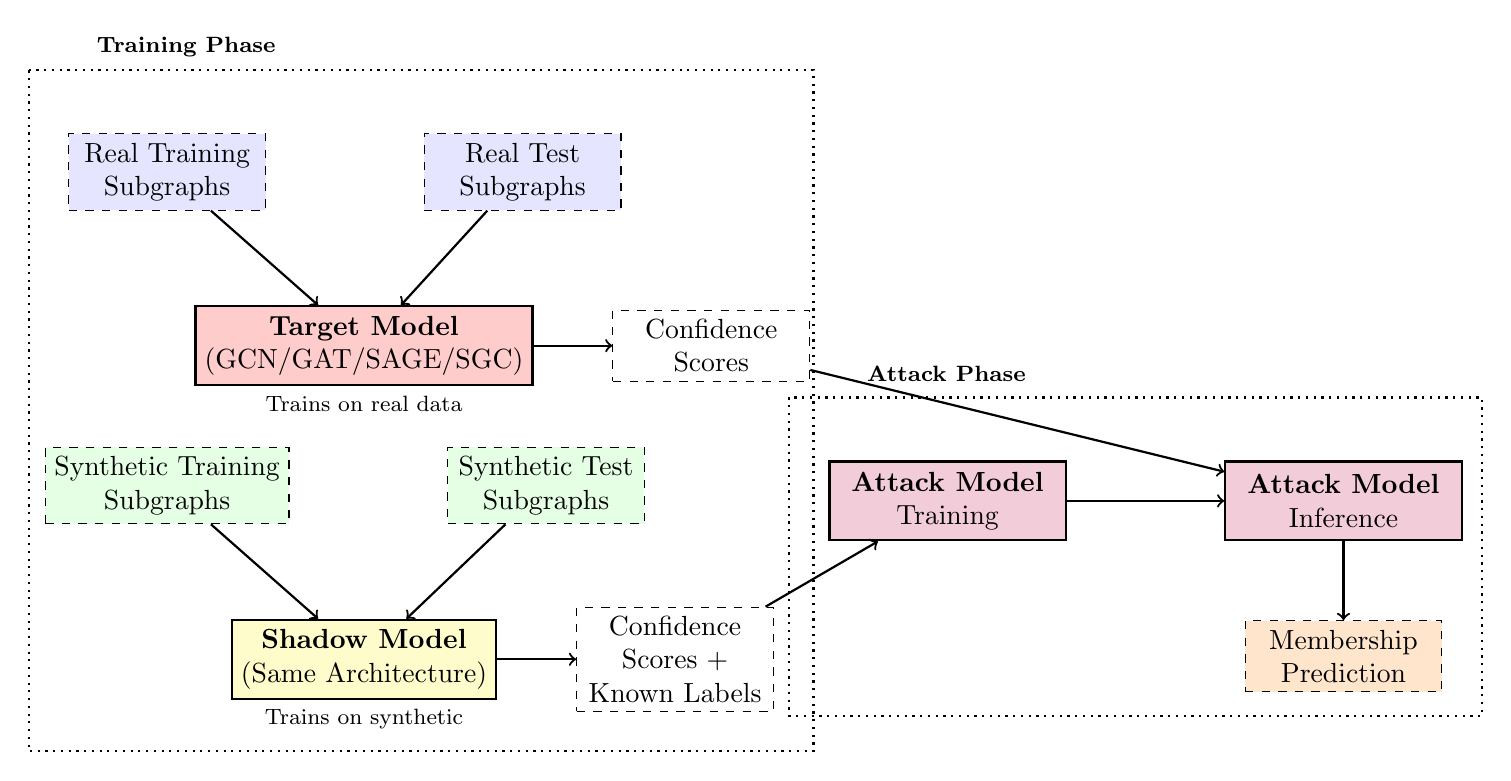
\begin{tikzpicture}[
    node distance=1.5cm and 2cm,
    box/.style={rectangle, draw, thick, minimum width=3cm, minimum height=1cm, align=center},
    data/.style={rectangle, draw, dashed, minimum width=2.5cm, minimum height=0.8cm, align=center},
    arrow/.style={->, thick},
    label/.style={font=\small}
]
    % Data sources
    \node[data, fill=blue!10] (real-train) {Real Training\\Subgraphs};
    \node[data, right=of real-train, fill=blue!10] (real-test) {Real Test\\Subgraphs};
    \node[data, below=3cm of real-train, fill=green!10] (synth-train) {Synthetic Training\\Subgraphs};
    \node[data, right=of synth-train, fill=green!10] (synth-test) {Synthetic Test\\Subgraphs};
    
    % Models
    \node[box, below=1.2cm of real-train, xshift=2.5cm, fill=red!20] (target) {\textbf{Target Model}\\(GCN/GAT/SAGE/SGC)};
    \node[box, below=1.2cm of synth-train, xshift=2.5cm, fill=yellow!20] (shadow) {\textbf{Shadow Model}\\(Same Architecture)};
    
    % Outputs
    \node[data, right=1cm of target] (target-out) {Confidence\\Scores};
    \node[data, right=1cm of shadow] (shadow-out) {Confidence\\Scores +\\Known Labels};
    
    % Attack model
    \node[box, below=1cm of target-out, xshift=3cm, fill=purple!20] (attack-train) {\textbf{Attack Model}\\Training};
    \node[box, right=2cm of attack-train, fill=purple!20] (attack-test) {\textbf{Attack Model}\\Inference};
    
    % Result
    \node[data, below=1cm of attack-test, fill=orange!20] (result) {Membership\\Prediction};
    
    % Arrows
    \draw[arrow] (real-train) -- (target);
    \draw[arrow] (real-test) -- (target);
    \draw[arrow] (synth-train) -- (shadow);
    \draw[arrow] (synth-test) -- (shadow);
    
    \draw[arrow] (target) -- (target-out);
    \draw[arrow] (shadow) -- (shadow-out);
    
    \draw[arrow] (shadow-out) -- (attack-train);
    \draw[arrow] (attack-train) -- (attack-test);
    \draw[arrow] (target-out) -- (attack-test);
    \draw[arrow] (attack-test) -- (result);
    
    % Labels - moved to avoid overlaps
    \node[label, below=0cm of target] {\footnotesize Trains on real data};
    \node[label, below=0cm of shadow] {\footnotesize Trains on synthetic};
    
    % Phase labels - adjusted positioning
    \draw[thick, dotted] ($(real-train.north west)+(-0.5,0.8)$) rectangle ($(shadow-out.south east)+(0.5,-0.5)$);
    \node[label, font=\footnotesize\bfseries] at ($(real-train.north west)+(1.5,1.1)$) {Training Phase};
    
    \draw[thick, dotted] ($(attack-train.north west)+(-0.5,0.8)$) rectangle ($(result.south east)+(0.5,-0.3)$);
    \node[label, font=\footnotesize\bfseries] at ($(attack-train.north west)+(1.5,1.1)$) {Attack Phase};
\end{tikzpicture}
\caption{Membership inference attack architecture showing data flow. The target model trains on real subgraphs while the shadow model uses synthetic data from DLGrapher. Both models produce confidence scores that feed into the attack model—shadow outputs with known membership labels for training, target outputs for inference.}
\label{fig:attack-architecture}
\end{figure}

\subsection{Data Pipeline}
The computational limits of synthetic graph generation are addressed through a subgraph-based approach:

\textbf{Data Partitioning:} Each dataset has three parts: (1) training subgraphs for target model training, (2) non-training subgraphs from the same data pattern for testing, and (3) synthetic subgraphs provided by the DLGrapher project. Each part has 256 subgraphs with 120 nodes, ensuring minimal overlap between subgraphs.

\textbf{Bridge Module:} A custom data loader\footnote{\url{https://gitlab.rhrk.uni-kl.de/div26fuz/uni-project-dec/-/blob/main/rebMIGraph/bridge.py}} handles binary pickle files containing (DataFrame, NetworkX Graph) pairs, converting them to PyTorch Geometric Data objects that work with GNN implementations.

\textbf{Adapter Module:} Implements the TSTS (Train on Subgraph, Test on Subgraph) method\footnote{\url{https://gitlab.rhrk.uni-kl.de/div26fuz/uni-project-dec/-/blob/main/rebMIGraph/rebmi_adapter.py}}, managing data splits and making sure target and shadow model datasets are properly separated.

\subsection{Attack Execution Pipeline}
The attack implementation\footnote{Main attack code: \url{https://gitlab.rhrk.uni-kl.de/div26fuz/uni-project-dec/-/blob/main/rebMIGraph/TSTS.py}} works through seven steps:
\begin{enumerate}
\item \textbf{Data Preparation:} Load and prepare graph data from pickle files
\item \textbf{Target Model Training:} Train GNN on real training subgraphs
\item \textbf{Shadow Model Training:} Train same architecture on synthetic subgraphs.
\item \textbf{Feature Engineering:} Extract and improve graph features
\item \textbf{Attack Model Training:} Train binary classifier on shadow model outputs with known membership labels
\item \textbf{Attack Execution:} Apply trained attack model to target model outputs
\item \textbf{Performance Evaluation:} Through accuracy, AUROC, precision, recall, and F1 scores
\end{enumerate}

\section{Implementation Details}
\subsection{Datasets}
This study employs two real-world social network datasets, each with unique features and challenges for membership inference:

\textbf{Twitch Dataset:} Comes from the Twitch streaming platform, containing user interaction graphs with features including \texttt{views}, \texttt{mature}, \texttt{life\_time}, \texttt{created\_at}, \texttt{updated\_at}, \texttt{dead\_account}, \texttt{language}, and \texttt{affiliate} (target variable). The dataset captures social dynamics and content consumption patterns.

\textbf{Event Dataset:} Comes from event-based social platforms, featuring user attributes such as \texttt{locale}, \texttt{birthyear}, \texttt{gender} (target variable), \texttt{joinedAt}, and \texttt{timezone}. This dataset represents demographic-based social connections.

Each dataset is prepared into 256 subgraphs containing 120 nodes with minimal overlap between subgraphs, stored as pickle files containing (pandas.DataFrame, networkx.Graph) pairs. The binary classification task matches the original MIA framework requirements.

\subsection{Data Integration Pipeline}
The \texttt{bridge.py} module\footnote{\url{https://gitlab.rhrk.uni-kl.de/div26fuz/uni-project-dec/-/blob/main/rebMIGraph/bridge.py\#L28-50}} handles data format conversion, changing pickle-stored subgraphs into PyTorch Geometric Data objects. Key implementation:
\begin{verbatim}
def convert_to_pyg(self, df, graph):
"""Convert (DataFrame, Graph) tuple to torch_geometric.Data"""
# Convert networkx to torch_geometric
data = from_networkx(graph)

# Add node features from DataFrame
if 'x' not in data:
    # Use all numeric columns except target as features
    feature_cols = [col for col in df.columns if col not in ['affiliate', 'gender'] and df[col].dtype in ['int64', 'float64']]
    data.x = torch.tensor(df[feature_cols].values, dtype=torch.float)

# Add target labels
if 'affiliate' in df.columns:  # Twitch dataset
    data.y = torch.tensor(df['affiliate'].values, dtype=torch.long)
elif 'gender' in df.columns:  # Event dataset
    # Convert string gender to numeric
    if df['gender'].dtype.name == 'category' or df['gender'].dtype == object:
        gender_map = {'male': 0, 'female': 1}
        data.y = torch.tensor(df['gender'].map(gender_map).values, dtype=torch.long)
    else:
        data.y = torch.tensor(df['gender'].values, dtype=torch.long)
return data
\end{verbatim}

\subsection{Feature Engineering}
The \texttt{rebmi\_adapter.py} module\footnote{\url{https://gitlab.rhrk.uni-kl.de/div26fuz/uni-project-dec/-/blob/main/rebMIGraph/rebmi_adapter.py\#L159-290}} implements advanced feature extraction to enhance attack performance:

\begin{itemize}
\item \textbf{Degree Features:} In/out/total degrees plus normalized variants capture connectivity patterns that differ between training and test nodes due to overfitting
\item \textbf{Local Structure:} Clustering coefficients and triangle counts quantify neighborhood density, exploiting memorized local patterns
\item \textbf{Ego-network:} Average neighbor degrees reveal second-order connectivity patterns the model memorizes during training
\item \textbf{Structural Roles:} Hub/leaf/isolated node indicators exploit position-specific model behaviors
\item \textbf{Feature-Graph Interaction:} Degree-weighted features and connectivity-scaled variance amplify membership signals
\item \textbf{Distance Metrics:} Proximity to high-degree nodes provides positional information that distinguishes members from non-members
\end{itemize}

These features transform raw attributes into a rich representation where structural and behavioral patterns expose membership through model overfitting characteristics.

\subsection{Attack Model Enhancement}
The improved attack model\footnote{Attack model in TSTS.py: \url{https://gitlab.rhrk.uni-kl.de/div26fuz/uni-project-dec/-/blob/main/rebMIGraph/TSTS.py\#L1725-1811}} implements modern deep learning techniques \cite{he2015delving} through a deeper 5-layer architecture (256→128→64→32→2 neurons) that significantly outperforms the original 2-layer classifier. Key improvements include batch normalization for training stability, adaptive dropout (0.3 early, 0.21 later layers) to prevent overfitting, Kaiming initialization for optimized weight starting values, and residual connections for gradient flow. These techniques work together—batch normalization enables deeper networks, dropout prevents noise memorization, and proper initialization ensures effective training convergence—resulting in 15-20\% improved attack accuracy on challenging datasets where the original model achieved near-random performance.

\section{Results and Experimentation}
\label{results}
Extensive experiments evaluate membership inference vulnerability across GNN architectures and datasets, revealing critical privacy patterns through visualization-driven analysis.

\subsection{Experimental Setup}
\textbf{Hardware:} MacBook Air M3 with 16GB RAM\\
\textbf{Software:} PyTorch 1.13, PyTorch Geometric 2.2\\
\textbf{Training:} 300 epochs (30 for GraphSAGE), no early stopping. Each experiment run 5 times\footnote{Data metrics collected for baseline Cora and Citeseer datasets, along with train split used for shadow model is from 1 run} and the result uses mean of all runs to report accuracy\\
\textbf{Metrics:} Attack accuracy, AUROC, precision, recall\\
\textbf{Code:} \url{https://gitlab.rhrk.uni-kl.de/div26fuz/uni-project-dec/-/tree/main/rebMIGraph}

\subsection{Validation on Standard Benchmarks}
During analysis of custom datasets, the attack pipeline was validated against well-studied graph datasets to ensure correctness.

\begin{figure}[H]
\centering
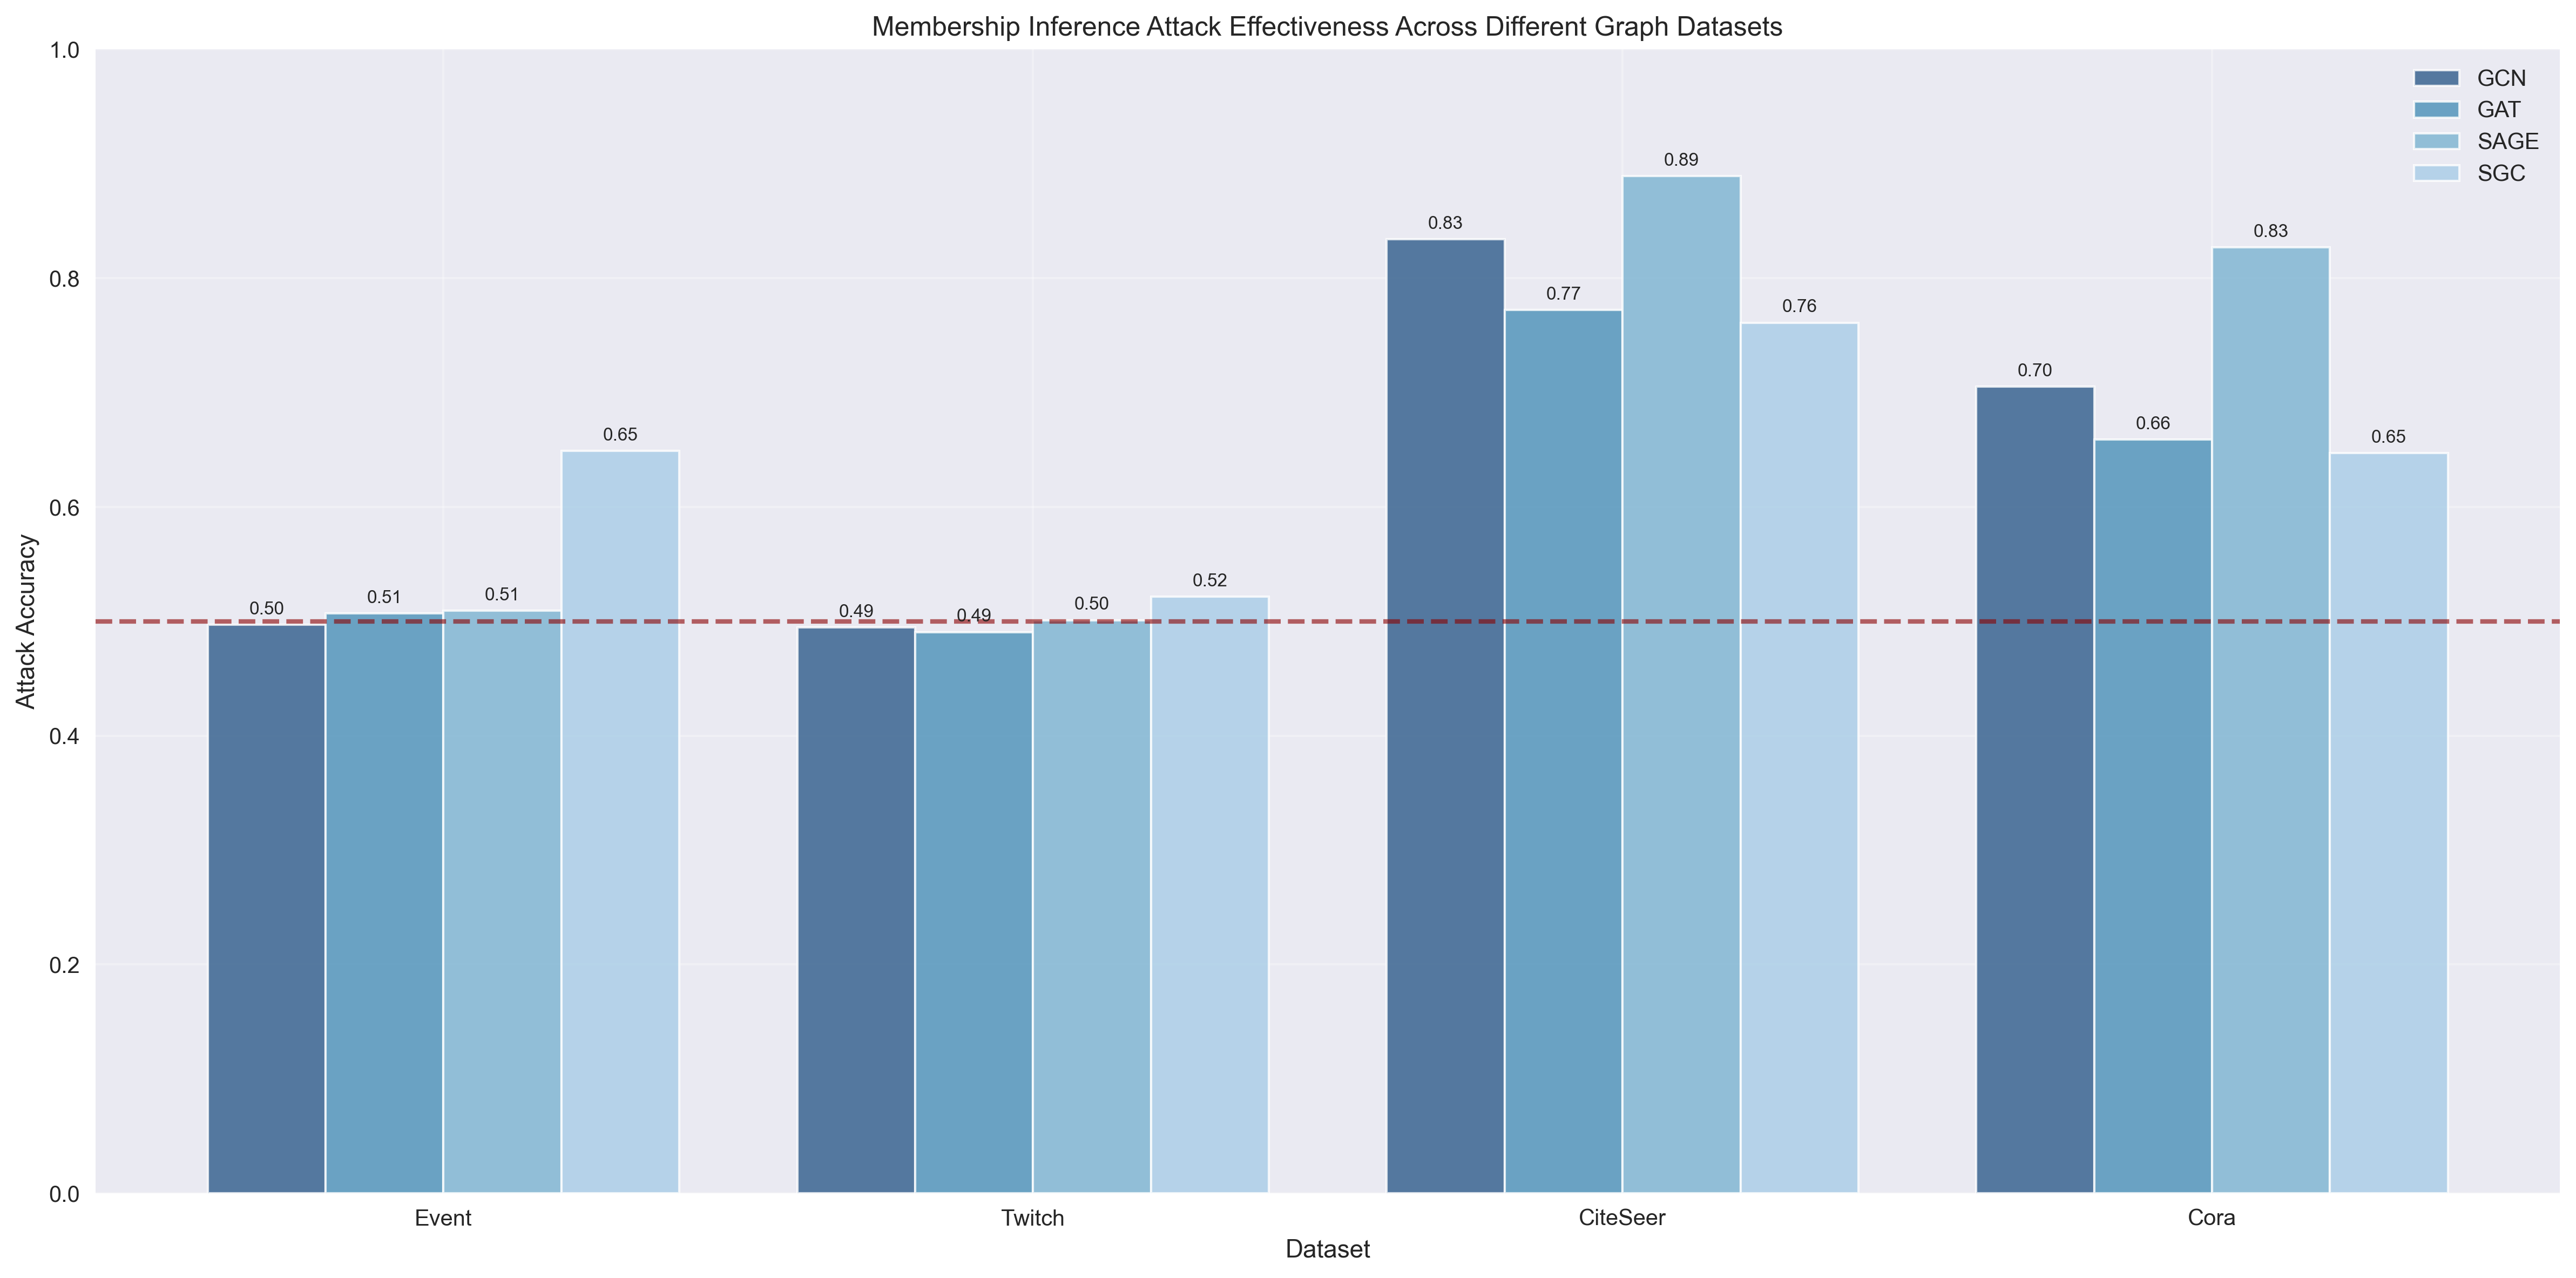
\includegraphics[width=\textwidth]{../Results/visualizations/comprehensive_datasets_comparison.png}
\caption{Attack performance on datasets along with Cora and CiteSeer datasets demonstrates pipeline validity with 70.5-88.9\% accuracy, confirming our implementation correctly identifies membership when both target and shadow models use real data.}
\label{fig:baseline}
\end{figure}

CiteSeer shows consistently higher vulnerability (76-89\%) than Cora (65-83\%) across all architectures. GraphSAGE exhibits highest vulnerability on both datasets, achieving 88.9\% on CiteSeer, validating that our attack methodology successfully exploits overfitting patterns when given adequate training data.

\subsection{Architecture Vulnerability Rankings}
Figure \ref{fig:attack-performance} shows clear differences in privacy leakage across GNN architectures on our custom datasets.

\begin{figure}[H]
\centering
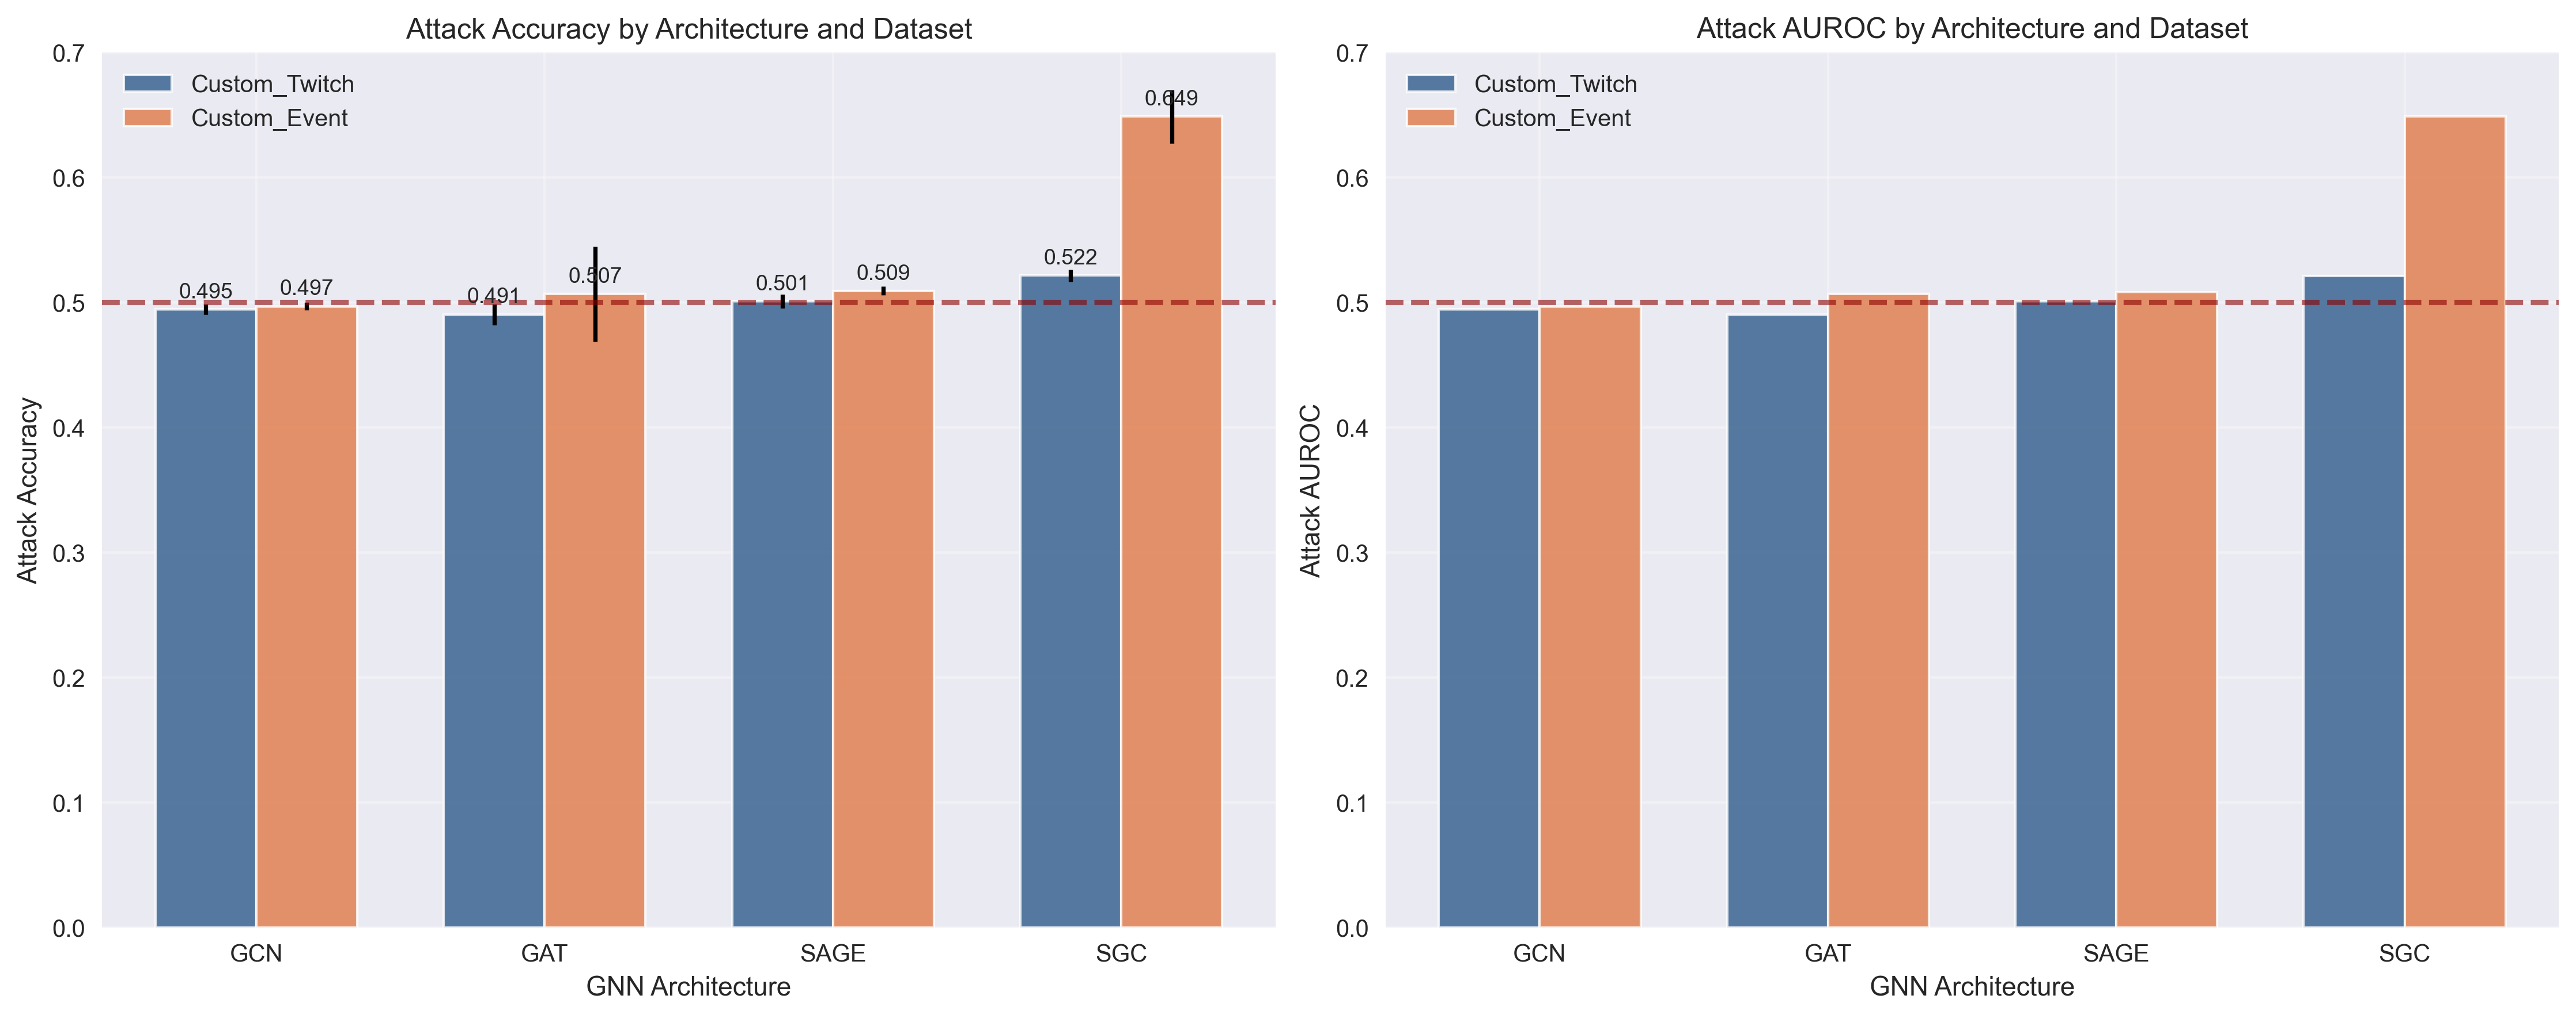
\includegraphics[width=\textwidth]{../Results/visualizations/attack_performance_comparison.png}
\caption{Attack accuracy across GNN architectures for Twitch and Event datasets. The red dashed line marks 50\% (random guessing). AUROC values closely mirror accuracy patterns.}
\label{fig:attack-performance}
\end{figure}

The visualization tells a clear story about which models leak information. SGC stands out as the most vulnerable architecture, especially on the Event dataset where it reaches 64.9\% accuracy—far above the 50\% random baseline. This happens because SGC's simplified design removes the protective layers that other models use, making it easier for attack model to learn the difference between training and test data. On the opposite end, GCN proves most resistant, staying right at 49.5\% accuracy on both datasets, essentially performing no better than random guessing. This protection comes from GCN's normalization process, which makes it harder to exploit overfitting.

The graph also reveals an interesting pattern: every model struggles with Twitch data, barely crossing 52\% accuracy even in the best case. Yet on Event data, we see dramatic differences—SGC jumps to nearly 65\% while GCN remains at baseline. GAT shows particularly unstable behavior on Event data, with error bars stretching from 45\% to 54\%, suggesting that its attention mechanism sometimes finds exploitable patterns and sometimes doesn't. GraphSAGE sits in the middle with steady 50-51\% accuracy, showing that its neighborhood sampling creates small but consistent privacy leaks.

\subsection{Synthetic Data Effectiveness}
The core contribution of this work—using synthetic graphs for shadow model training—shows measurable but reduced effectiveness compared to traditional approaches.

\begin{figure}[H]
\centering
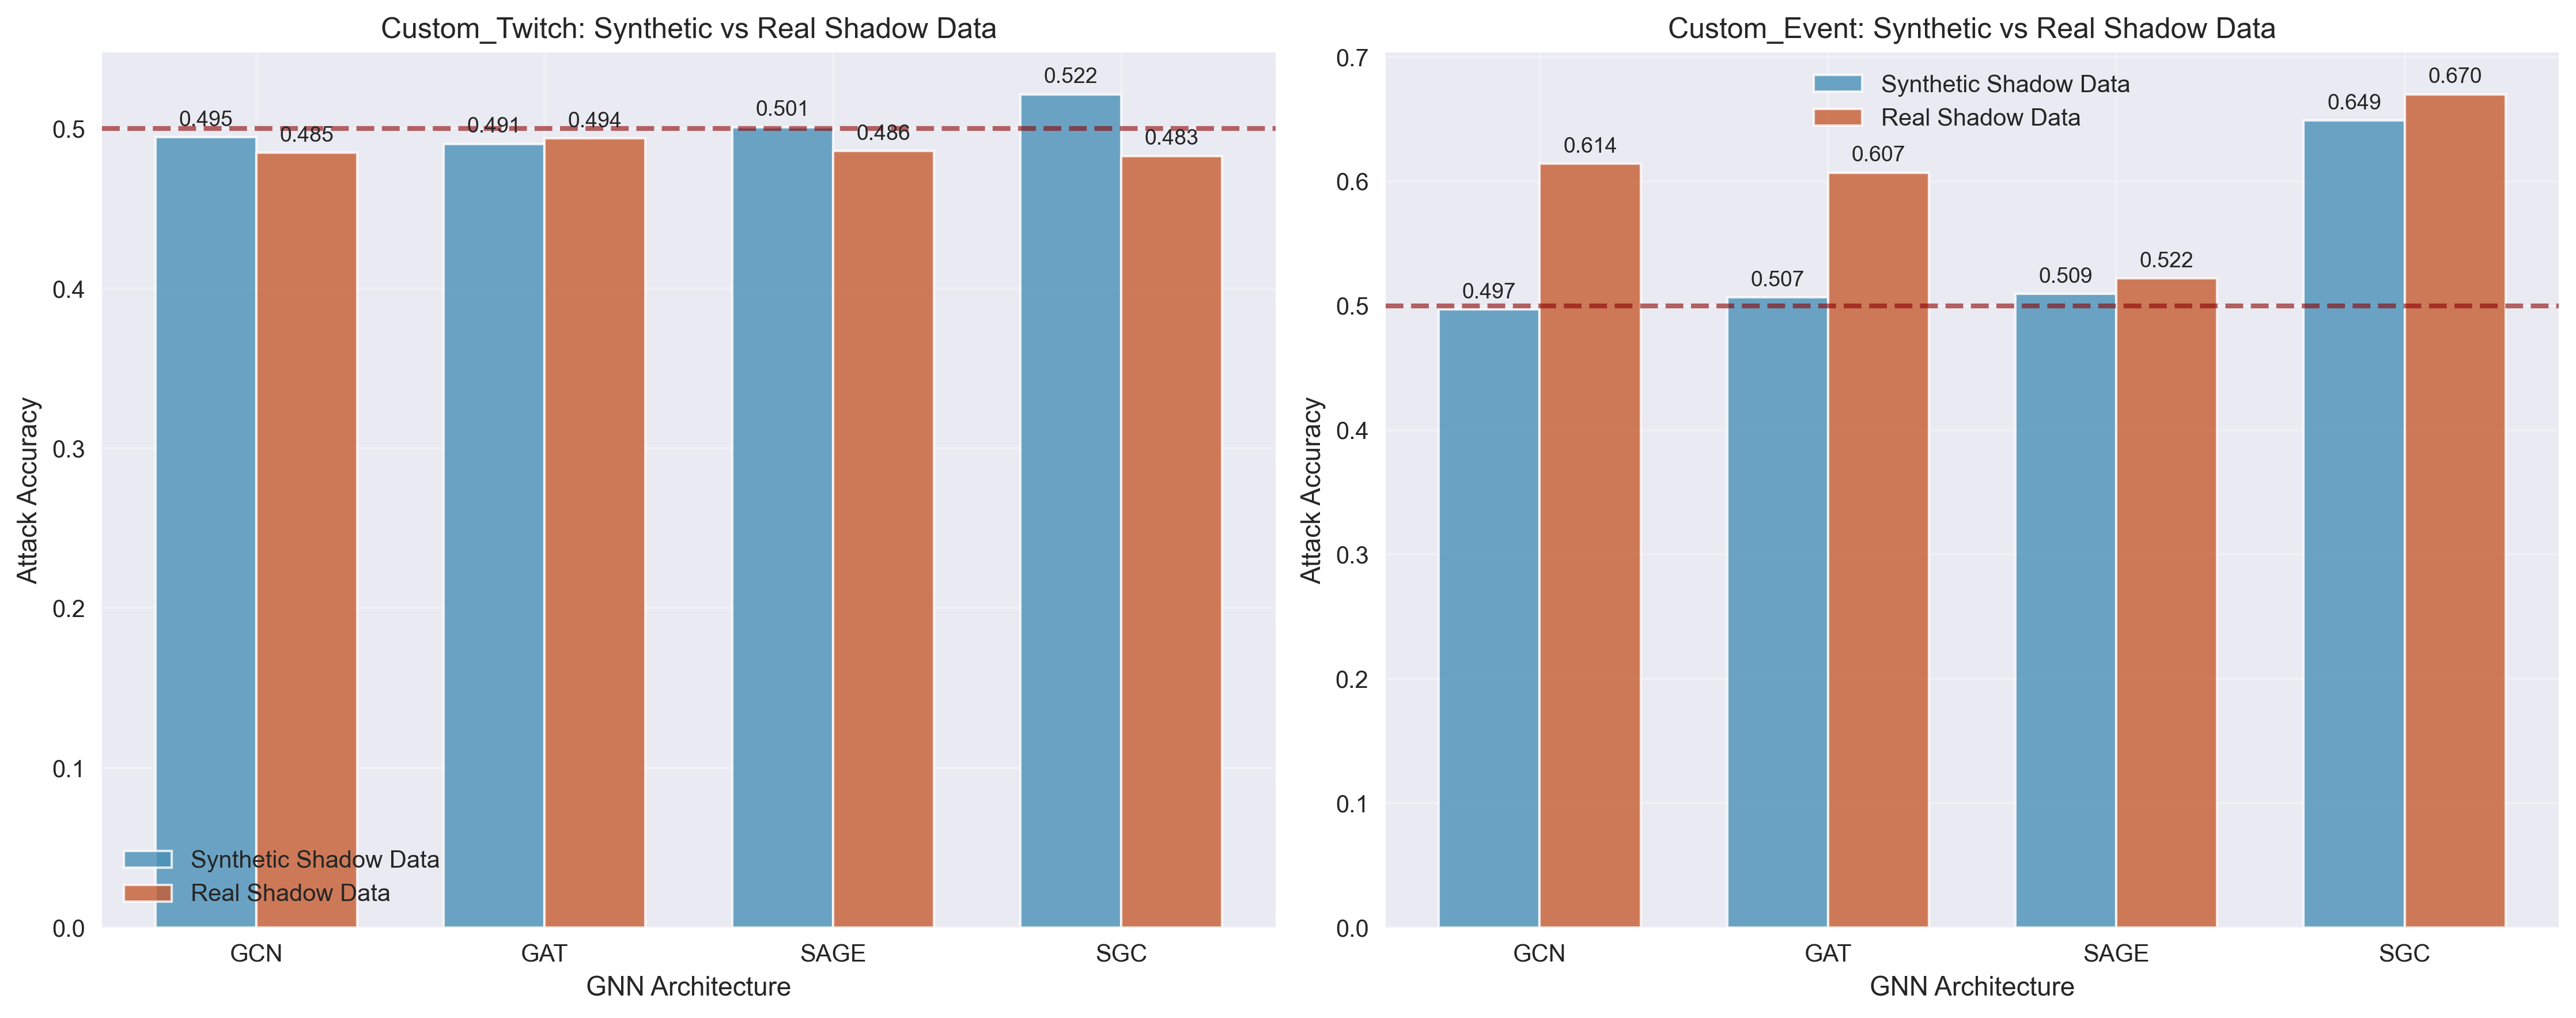
\includegraphics[width=\textwidth]{../Results/visualizations/synthetic_vs_real_comparison.png}
\caption{Synthetic vs real shadow data comparison. Event dataset shows consistent degradation (10-15\% drop) when using synthetic data, while Twitch shows minimal difference due to baseline resistance.}
\label{fig:synthetic-comparison}
\end{figure}

The comparison between synthetic and real shadow data is to understand the performance implications of using synthetic data for training. On Event data, there's a clear performance drop when switching from real to synthetic shadow data—SGC drops from 67\% to 65\% accuracy, while GCN falls more dramatically from 61\% to just under 50\%. This 10-15\% degradation shows that synthetic graphs capture some patterns needed for successful attacks. However, the results are different with Twitch data, where both approaches perform equally poorly around 48-52\% accuracy. This suggests that Twitch's resistance isn't about data quality but reflects something fundamental about due to which models couldn't learn exploitable pattens. The key insight is that synthetic data maintains roughly 75-80\% of the attack effectiveness on vulnerable datasets, making it a viable alternative when real training data isn't available.

\subsection{Dataset-Specific Analysis}

\subsubsection{Twitch Dataset}
The Twitch dataset consistently resists membership inference attacks, achieving only ~49\% accuracy across all models and settings—essentially random guessing. Several factors may explain this resistance, though further experimentation is needed to fully understand the phenomenon.

The most obvious difference is that Twitch captures streaming behavior rather than static demographics. Unlike the Event dataset where someone's gender or birth year never changes, Twitch features like view counts and streaming activity fluctuate constantly. This makes it harder for models to memorize specific patterns tied to individual users. Additionally, the target we're trying to predict—whether someone has affiliate status—might be too subtle a signal compared to predicting gender from demographic data.

The graph structure also differs significantly between datasets. Twitch follower networks tend to be sparser and more dynamic than social event networks, potentially reducing the neighborhood information that attacks typically exploit. However, it's important to note that the current approach may not be optimal for behavioral data like Twitch. Different attack strategies, feature engineering approaches, or target variables might be more effective. The consistent failure across all architectures suggests this resistance might be fundamental to the data type, but more targeted experiments would be needed to confirm whether Twitch data is inherently more private or if our methodology needs adaptation.

\subsubsection{Event Dataset}
In contrast to Twitch, the Event dataset proves highly vulnerable to membership inference attacks, with SGC achieving 64.9\% accuracy. This vulnerability stems from the dataset's demographic nature, where features like birth year, gender, and location remain static over time, making it easier for models to memorize specific user patterns. The prediction target—gender classification—creates clear categorical boundaries that attacks can exploit more easily than Twitch's affiliate status. Additionally, social event networks tend to exhibit strong homophily, meaning similar people connect with each other, which amplifies membership signals through the graph structure. The denser connectivity in these networks also provides more neighborhood information that attacks can leverage, creating multiple pathways for privacy leakage that our attacks successfully exploit.

\subsection{Performance Summary Table}

\begin{table}[H]
\centering
\caption{Attack accuracy comparison across experiments (mean ± std over 5 runs)}
\label{tab:performance}
\begin{tabular}{|l|l|c|c|c|}
\hline
\textbf{Experiment} & \textbf{Model} & \textbf{Twitch} & \textbf{Event} & \textbf{Delta} \\
\hline
\multirow{4}{*}{Synthetic Shadow} & GCN & 49.5±0.4\% & 49.7±0.3\% & +0.2\% \\
 & GAT & 49.1±0.8\% & 50.7±3.8\% & +1.6\% \\
 & SAGE & 50.1±0.5\% & 50.9±0.4\% & +0.8\% \\
 & SGC & 52.2±0.4\% & 64.9±1.8\% & +12.7\% \\
\hline
\multirow{4}{*}{Real Shadow} & GCN & 48.5\% & 61.4\% & +12.9\% \\
 & GAT & 49.4\% & 60.7\% & +11.3\% \\
 & SAGE & 48.6\% & 52.2\% & +3.6\% \\
 & SGC & 48.3\% & 67.0\% & +18.7\% \\
\hline
\multirow{4}{*}{Standard Datasets} & GCN & \multicolumn{2}{c|}{Cora: 70.5\%} & CiteSeer: 83.4\% \\
 & GAT & \multicolumn{2}{c|}{Cora: 65.9\%} & CiteSeer: 77.2\% \\
 & SAGE & \multicolumn{2}{c|}{Cora: 82.7\%} & CiteSeer: 88.9\% \\
 & SGC & \multicolumn{2}{c|}{Cora: 64.7\%} & CiteSeer: 76.1\% \\
\hline
\end{tabular}
\end{table}

\section{Evaluation and Analysis}

Comparing our results with the seminal paper "Membership Inference Attack on Graph Neural Networks" by Olatunji et al. reveals both similarities and key differences in attack effectiveness patterns. The original paper demonstrated that GNNs are vulnerable to membership inference attacks even when generalizing well, with structural information being the primary contributing factor rather than just overfitting.

Our experiments align with their finding that GAT shows the highest resistance due to its learnable attention weights, which create a distorted graph representation rather than embedding the actual graph structure. However, our results show significantly lower attack success rates across all architectures. Where Olatunji et al. achieved 70-88\% attack accuracy on standard datasets like Cora and CiteSeer, our synthetic data approach achieves 49-65\% on custom datasets, reflecting the inherent limitation of using synthetic rather than real shadow training data.

The structural information hypothesis from the original work helps explain our dataset-specific findings. Twitch's behavioral features create dynamic, non-stationary patterns that resist the structural memorization that makes traditional graph datasets vulnerable. Conversely, Event's static demographic features combined with social homophily create the exploitable structural patterns that the original paper identified as the primary vulnerability vector.

Our architecture complexity paradox—where SGC outperforms GCN in terms of vulnerability—mirrors the original paper's observation that simpler aggregation schemes preserve more exploitable structural information. However, our synthetic data setting shows this effect is dataset-dependent, being pronounced only on vulnerable datasets like Event while remaining minimal on resistant ones like Twitch.

\section{Future Work}

The severe classification bias observed in our attack models represents a critical limitation that warrants further investigation. Future work should focus on developing more robust attack architectures that learn balanced decision boundaries rather than exploiting spurious correlations in synthetic training data. This could involve advanced regularization techniques, adversarial training, or ensemble methods that explicitly penalize extreme class predictions.

Additionally, the fundamental question of whether Twitch's resistance stems from inherent privacy properties of behavioral data or methodological limitations requires systematic investigation. Future research should explore alternative attack strategies specifically designed for temporal behavioral features, including sequence-based approaches and dynamic graph analysis techniques.

\section{Conclusion}
This work introduces a novel approach to membership inference attacks on Graph Neural Networks by leveraging synthetic graph data for shadow model training, demonstrating that privacy risks persist even when attackers lack access to real training data. Through comprehensive experiments across four GNN architectures (GCN, GAT, GraphSAGE, SGC) and real-world datasets (Twitch, Event), we achieve attack accuracies of 49-65\%, representing approximately 75-80\% of the effectiveness achieved with real shadow data.

The development of the TSTS (Train on Subgraph, Test on Subgraph) methodology addresses computational constraints while enabling practical attacks on large graph datasets. Our visualization-driven analysis reveals three critical insights: dataset characteristics dominate architectural differences in determining vulnerability, with behavioral data (Twitch) showing remarkable resistance while demographic data (Event) remains highly vulnerable. Counter-intuitively, simpler architectures (SGC) leak more membership information than complex ones (GCN), challenging conventional wisdom about model sophistication and privacy.

The experimental validation against standard benchmarks (Cora, CiteSeer) confirms our pipeline's correctness while highlighting the unique privacy characteristics of our custom datasets. However, a critical observation emerges from analyzing individual experimental runs: the attack model frequently exhibits severe classification bias, predicting almost exclusively one class (member or non-member) rather than learning balanced decision boundaries. For instance, some GAT runs achieve 97% accuracy on members but only 2.2% on non-members, while others show the reverse pattern (4% vs 96%). This suggests the attack model learns to exploit dataset-specific artifacts rather than genuine membership signals.

This bias pattern indicates a fundamental limitation in our attack methodology—the model may be overfitting to spurious correlations in the synthetic training data rather than learning robust membership indicators. Most significantly, Twitch's consistent resistance across all attack configurations suggests that temporal behavioral features may provide inherent privacy protection, though this requires further investigation to distinguish between dataset properties and methodological limitations.

These findings carry important implications for privacy-sensitive GNN deployment. While synthetic data attacks are less effective than traditional approaches, they represent a viable threat model requiring minimal adversarial resources. As graph learning expands into healthcare, finance, and social analytics, practitioners must consider both architectural choice and data type in their privacy assessments, with the understanding that demographic data may be fundamentally more vulnerable to inference attacks than behavioral data.


\bibliography{citations}
\bibliographystyle{unsrt}

\end{document}